\begin{frame}
    \frametitle{A Man of Focus, Commitment and Sheer Freaking Will}
      \begin{figure}[!htbp]
        \centering
        % \captionsetup{justification=centering}
        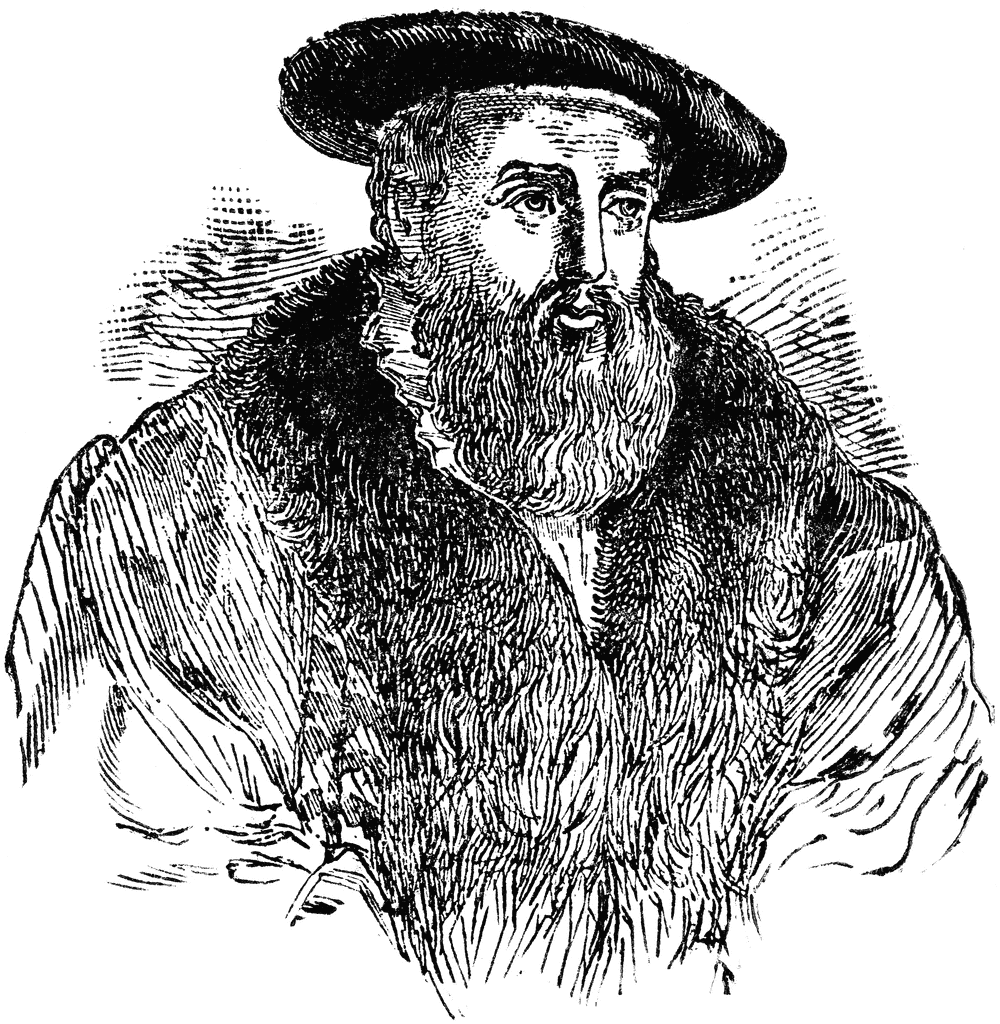
\includegraphics[width=0.5\textwidth]{./data/image/kepler.png}
      \caption{Johannes Kepler(1571--1630)}
      \label{image:kepler}
      \end{figure}
    \end{frame}
    
    \begin{frame}
      \frametitle{Kepler's Laws of Planetary Motion}
      \pause
      After working with Tycho Brahe's(1546--1601) data for around 8--9 years in 1609 Kepler publishes the first two laws as:
      \begin{itemize}
        \pause
        \item The orbit of a planet is an ellipse with the Sun at one of the two foci.
        \pause
        \item A line segment joining a planet and the Sun sweeps out equal areas during equal intervals of time.
      \end{itemize}
      \pause
        \begin{figure}
          \centering
          % \captionsetup{justification=centering}
          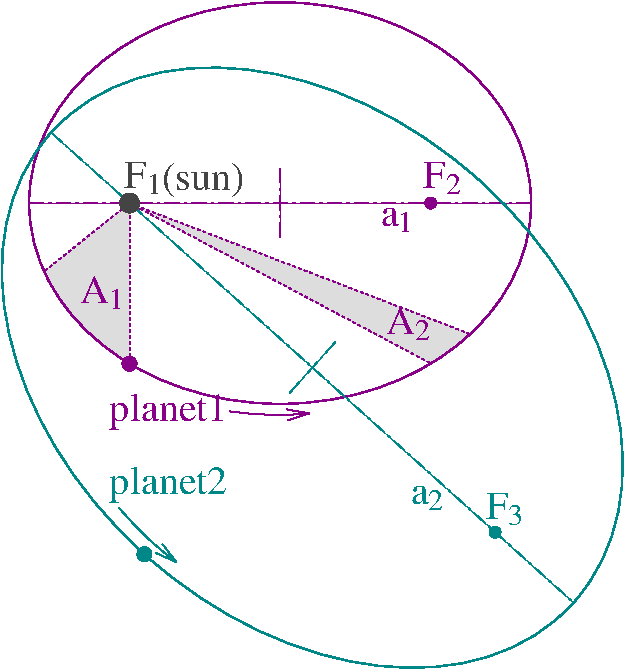
\includegraphics[width=0.35\textwidth]{./data/image/kepler_laws_diagram.pdf}
        \caption{Visualization of The Kepler's Laws}
        % \label{image:kepleanetary}
        \end{figure}
      \end{frame}
      \begin{frame}
        \frametitle{Kepler's Luck and Years of Perseverance}
        \pause
        Kepler got lucky by reading John Napier(1550--1617) paper on logarithm and after a ``mere'' 10 years of 
        excruciating pain came up with:
        \begin{itemize}
            \pause
          \item The square of a planet's orbital period is proportional to the cube of the length of the semi-major axis of its orbit.
        \end{itemize}
        \pause
          \begin{figure}
            \centering
            % \captionsetup{justification=centering}
            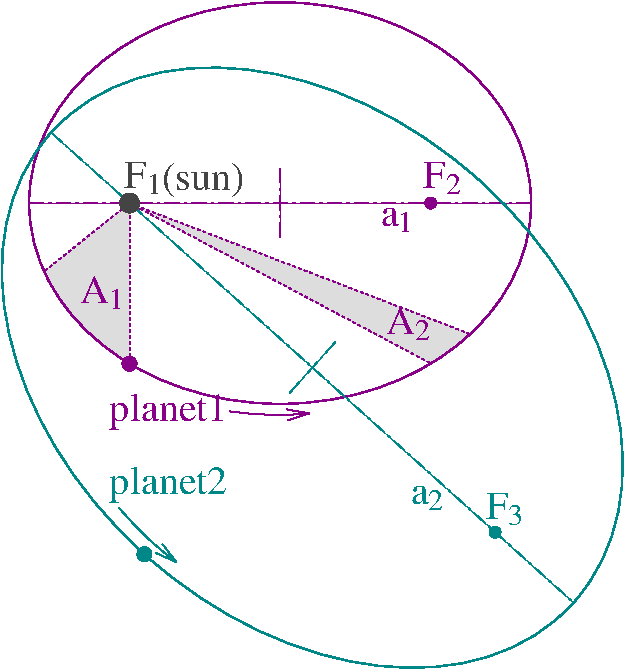
\includegraphics[width=0.35\textwidth]{./data/image/kepler_laws_diagram.pdf}
          \caption{Visualization of The Kepler's Laws}
          \label{image:kepler_luck_napier}
          \end{figure}
        \end{frame}
     
    
    

    
    
    
    
      \begin{frame}
        \frametitle{Kepler's Laws of Planetary Motion}
        And Finally in 1619
        \pause
        \begin{itemize}[<+->]
          \item The square of a planet's orbital period is proportional to the cube of the length of the semi-major axis of its orbit.
        \end{itemize}
        % \pause
          \begin{figure}
            \centering
            % \captionsetup{justification=centering}
            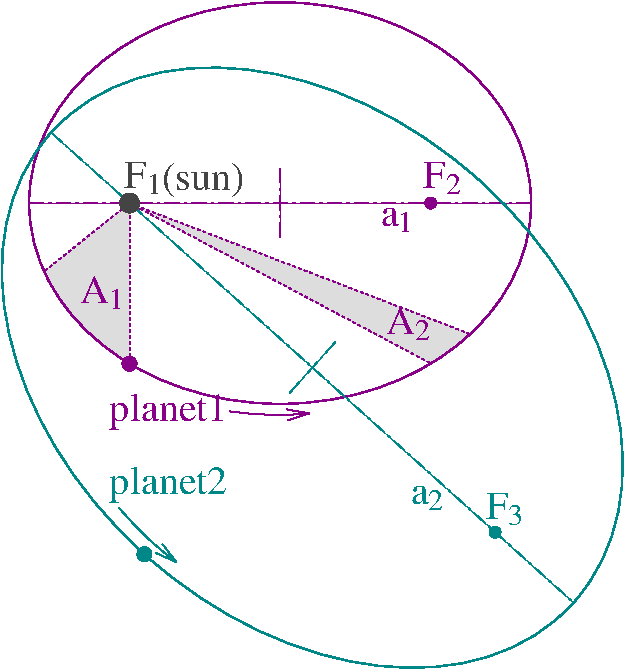
\includegraphics[width=0.35\textwidth]{./data/image/kepler_laws_diagram.pdf}
          \caption{Visualization of The Kepler's Laws}
          \label{image:kepler_law_planetary}
          \end{figure}
        \end{frame}
    
      \begin{frame}
        \frametitle{Kepler Doing Pseudo Linear Regression}
        \begin{Pro}
        If $T$ is the period of a planet in the solar system orbiting around the sun in earth-days and 
        $R$ is the average distance of the planets to sun over the average distance of the earth to sun,
         then find a $c$ that more or less explains 
        the observations below by the relation $T=cR^{3/2}$.
          
        \end{Pro}
        \begin{tabular}{|c|r|p{1.3cm}|p{2cm}|p{2cm}|p{2cm}|}
          \hline
          \multicolumn{4}{|c|}{Data used by Kepler} \\
          \hline
          Planet & Mean Distance to Sun (AU) & Period (days) &$\frac{R^3}{T^2}(10^{-6}\frac{\text{AU}^3}{\text{day}^2})$\\
          \hline
          Mercury   & 0.389   & 87.77    & 7.64 \\
          Venus     &   0.724 & 224.70   & 7.52 \\
          Earth     & 1.000   & 365.25   & 7.50 \\
          Mars      & 1.524   & 686.95   & 7.49 \\
          Jupiter   &   5.200 & 4332.65  & 7.49 \\
          Saturn    & 9.510   & 10759.20 & 7.43 \\
          \hline
         \end{tabular}\label{tab:kepler_tycho_data}
        \end{frame}
    
    
    
    
            \begin{frame}
              \frametitle{Two-Body Problem AKA Different Planetary Systems}
              \begin{tikzpicture}
                \begin{axis}[
                    title={Contours of $\frac{R^3}{T^2}$},
                    axis lines = left,
                    line width=1.5pt,
                    xlabel = \(R\),
                    ylabel = {\(T\)},
                    domain=1:4,
                    enlargelimits,
                    view={0}{90},
                ]
                    \addplot3 [
                         contour lua={levels={2,4,7.50,20}},
                        %  thick,
                    ] {x^3/y^2};
                \end{axis}
                \end{tikzpicture} 
              \end{frame}


\begin{frame}
\frametitle{Multi-Layer Perceptron}
\begin{Def}
Let $\boldsymbol{x} \in \mathbb{R}^n,\boldsymbol{y} \in \mathbb{R}^m, \boldsymbol{h}^l \in \mathbb{R}^{k_l}, \boldsymbol{W}^1 \in \mathbb{R}^{k_1 \times n}
, \boldsymbol{b}^1 \in \mathbb{R}^{k_1}, \boldsymbol{W}^{N+1} \in \mathbb{R}^{m \times k_N}, \mathbb{b}^m,\boldsymbol{W}^{l+1} \in \mathbb{R}^{k_l \times k_{l+1}}$ 
where $m,n,l,k_{l\in \left\{0,\ldots,N-1\right\}} \in \mathbb{N}$ and $\varphi \colon \mathbb{R} \to \mathbb{R}$ is a 
nonlinear function with certain properties. Multi-Layer Perceptron is consecutive mappings of the form:
\begin{equation}
\begin{split}
    h_i^{1}   &= \sigma \left( \sum_{j}^{} W_{ij}^{1}x_j + b_i^{1} \right)\\ 
            & \cdot\\
    h_i^{l+1} &= \sigma \left( \sum_{j}^{} W_{ij}^{l+1}h_j^l + b_i^{l+1} \right)\\
            & \cdot\\
    y_i^{}    &= \sigma \left( \sum_{j}^{} W_{ij}^{N+1}h_j^N + b_i^{N+1} \right)
\end{split}
\end{equation}
\end{Def}
\end{frame} 


\begin{frame}
\begin{figure}
    \frametitle{Multi-Layer Perceptron}
    \centering
    % \captionsetup{justification=centering}
    \resizebox{1.0\textwidth}{!}{  \begin{tikzpicture}[x=2.2cm,y=1.4cm]
    \message{^^JNeural network, shifted}
    \readlist\Nnod{3,4,4,4,3} % array of number of nodes per layer
    \readlist\Nstr{n,p,q,r,m} % array of string number of nodes per layer
    \readlist\Cstr{\strut x,h^{(\prev)},h^{(\prev)},h^{(\prev)},y} % array of coefficient symbol per layer
    \def\yshift{0.5} % shift last node for dots
    
    \message{^^J  Layer}
    \foreachitem \N \in \Nnod{ % loop over layers
      \def\lay{\Ncnt} % alias of index of current layer
      \pgfmathsetmacro\prev{int(\Ncnt-1)} % number of previous layer
      \message{\lay,}
      \foreach \i [evaluate={\c=int(\i==\N); \y=\N/2-\i-\c*\yshift;
                   \index=(\i<\N?int(\i):"\Nstr[\lay]");
                   \x=\lay; \n=\nstyle;}] in {1,...,\N}{ % loop over nodes
        % NODES
        \node[node \n] (N\lay-\i) at (\x,\y) {$\Cstr[\lay]_{\index}$};
        
        % CONNECTIONS
        \ifnum\lay>1 % connect to previous layer
          \foreach \j in {1,...,\Nnod[\prev]}{ % loop over nodes in previous layer
            \draw[connect arrow,white,line width=1.2] (N\prev-\j) -- (N\lay-\i);
            \draw[connect arrow] (N\prev-\j) -- (N\lay-\i);
            %\draw[connect] (N\prev-\j.0) -- (N\lay-\i.180); % connect to left
          }
        \fi % else: nothing to connect first layer
        
      }
      \path (N\lay-\N) --++ (0,1+\yshift) node[midway,scale=1.5] {$\vdots$};
    }
    
    % LABELS
    % \node[above=5,align=center,mygreen!60!black] at (N1-1.90) {input\\[-0.2em]layer};
    % \node[above=2,align=center,myblue!60!black] at (N3-1.90) {hidden layers};
    % \node[above=10,align=center,myred!60!black] at (N\Nnodlen-1.90) {output\\[-0.2em]layer};
    
  \end{tikzpicture}
  
  }
    \caption{$\boldsymbol{x} =\text{input},\boldsymbol{h}^j=\text{hidden variables},\boldsymbol{y}=\text{output}$}
    \label{fig:multi_layer_perceptron}
\end{figure}
\end{frame} 

\begin{frame}
    \frametitle{ML Nonlinearities}
    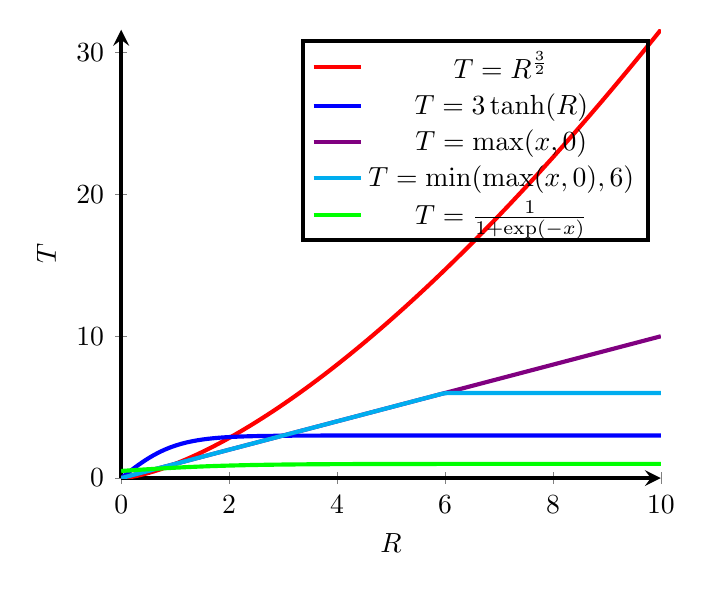
\begin{tikzpicture}
      \begin{axis}[
        legend style={fill=none},
        line width=1.5pt,
        % style sheet=vary hue,
          axis lines = left,
          xlabel = \(R\),
          ylabel = {\(T\)},
      ]
      %Below the red parabola is defined
      \addplot [
          domain=0:10, 
          samples=100, 
          color=red,
      ]
      {x^(3/2)};
      \addlegendentry{\(T = R^\frac{3}{2}\)}
      %Here the blue parabola is defined
      \addplot [
          domain=0:10, 
          samples=100, 
          color=blue,
          ]
          {3*tanh(x)};
      \addlegendentry{\(T = 3\tanh(R)\)}
      \addplot [
        domain=0:10, 
        samples=100, 
        color=violet,
        ]
        {max(0,x)};
    \addlegendentry{\(T = \max(x,0)\)}
    \addplot [
      domain=0:10, 
      samples=100, 
      color=cyan,
      ]
      {min(max(x,0),6)};
  \addlegendentry{\(T = \min(\max(x,0),6)\)}
  \addplot [
    domain=0:10, 
    samples=100, 
    color=green,
    ]
    { 1/(1+exp(-x)) };
\addlegendentry{\(T = \frac{1}{1+\exp(-x)}\)}
      \end{axis}
  \end{tikzpicture}
    \end{frame}








